\begin{figure}[!htb]
    \centering
    
    \Subfigure[0.3]{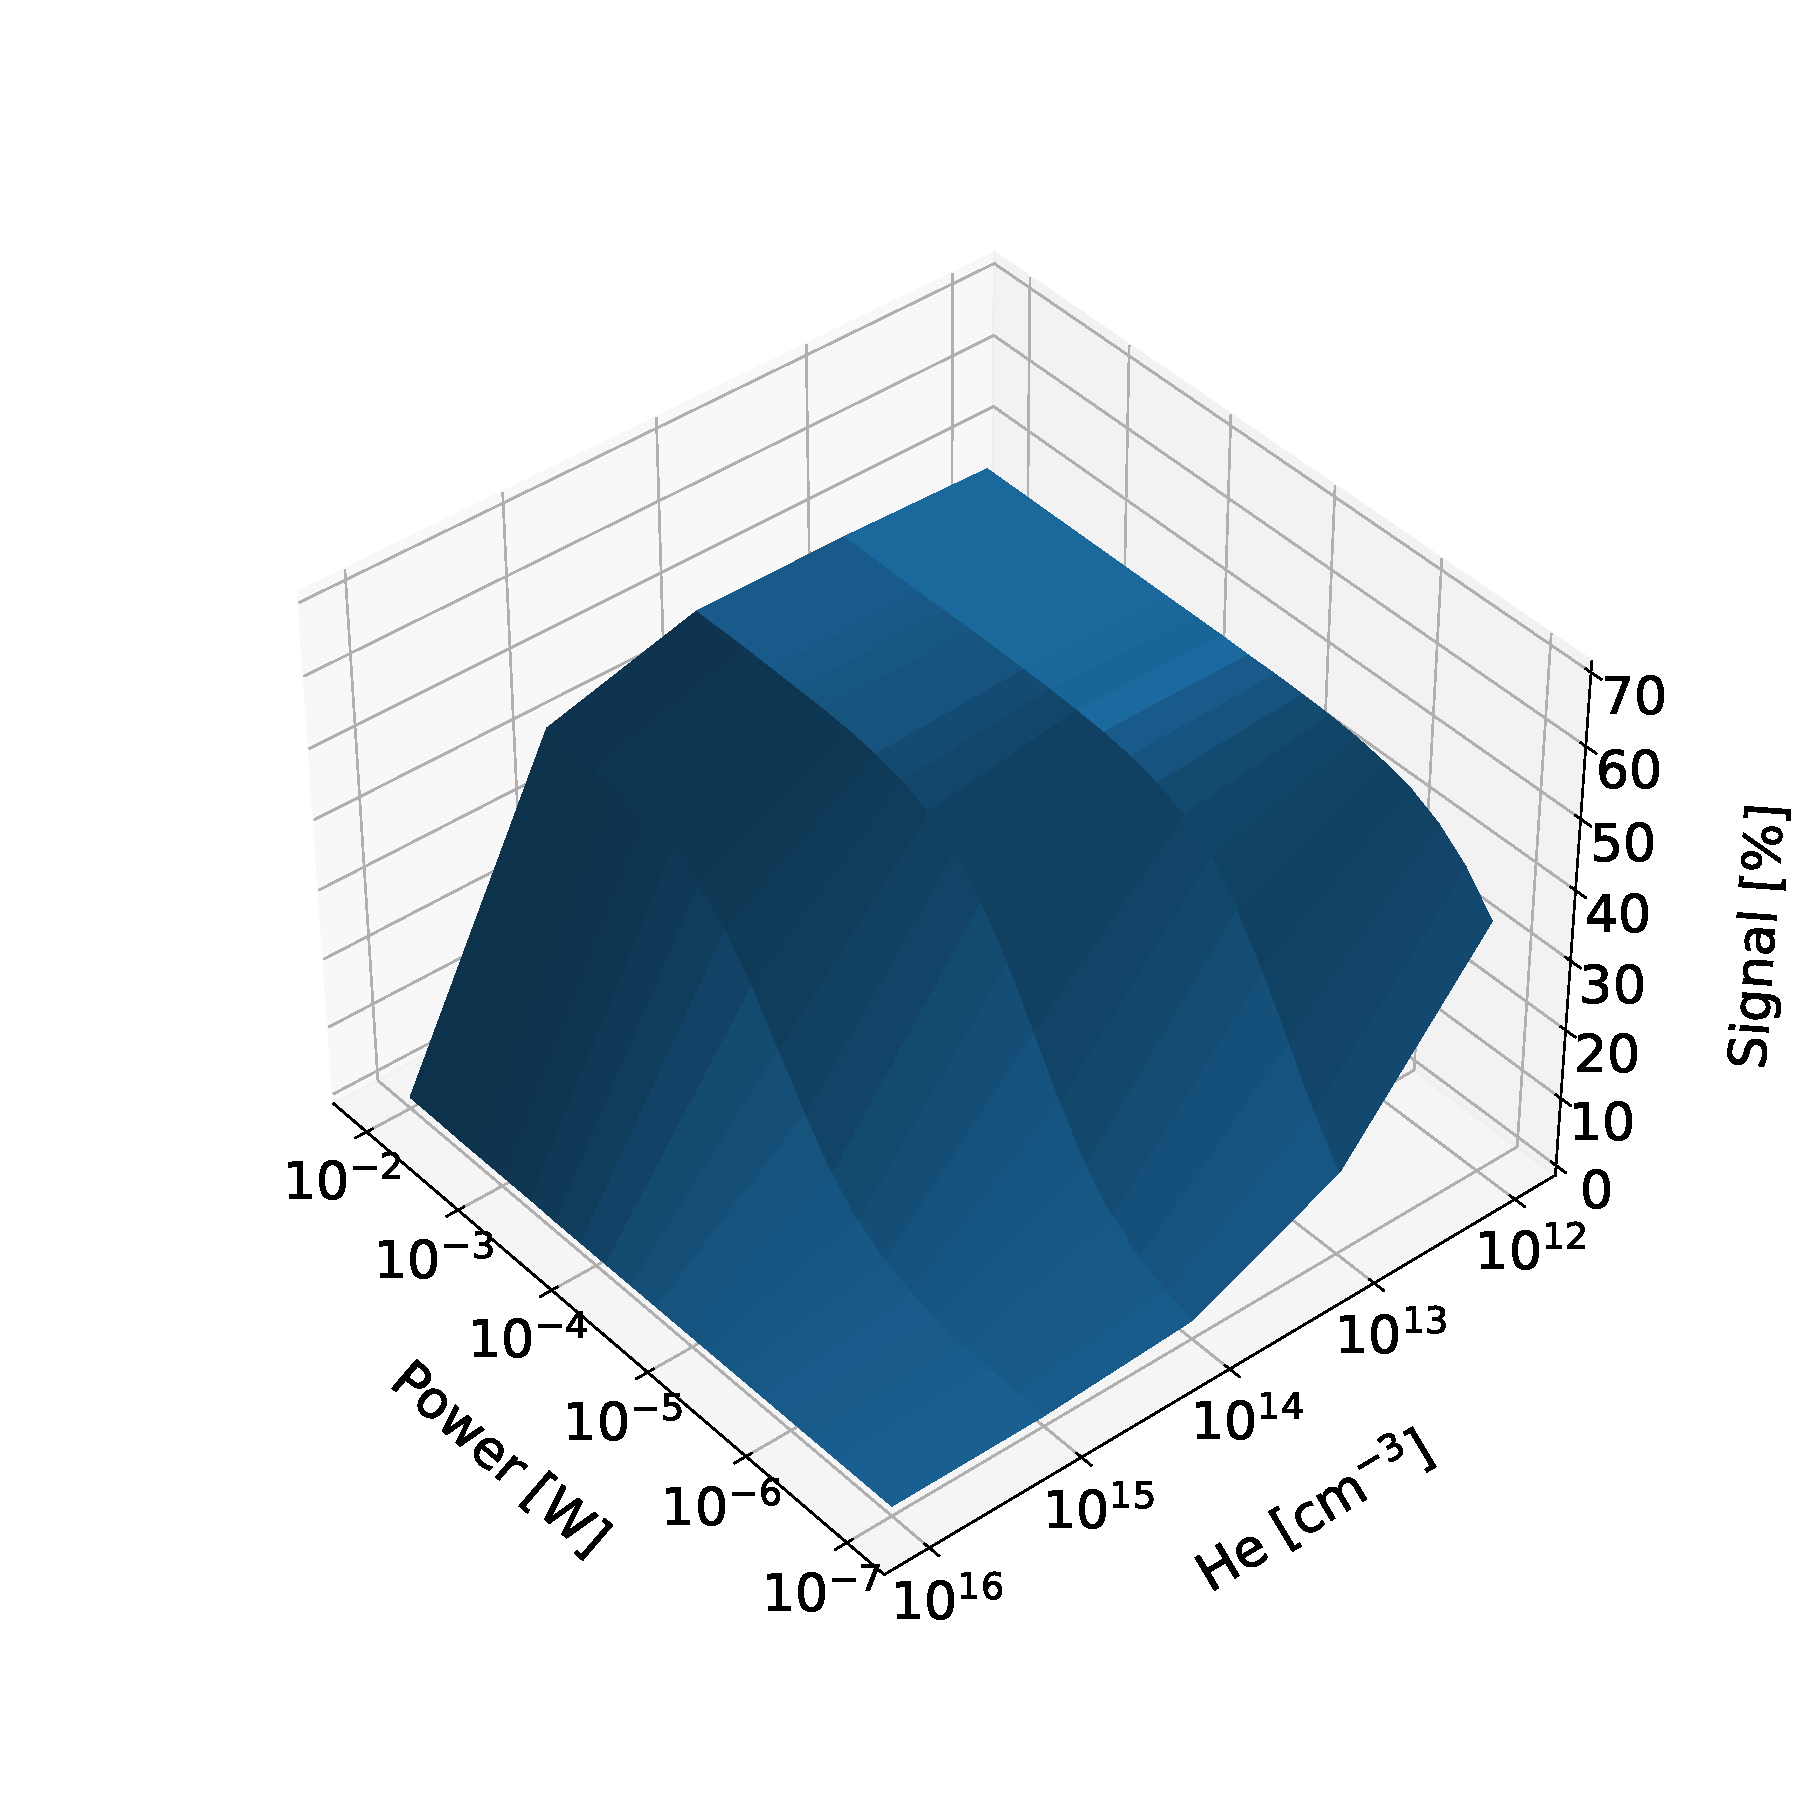
\includegraphics[width=1\textwidth]{figures/simulations/ROSAA/f-power_1e-7-1e-2/k3_branch_0.30.pdf}}{$k_{3_1}$ ratio $=0.3$}{}
    \hfill
    \Subfigure[0.3]{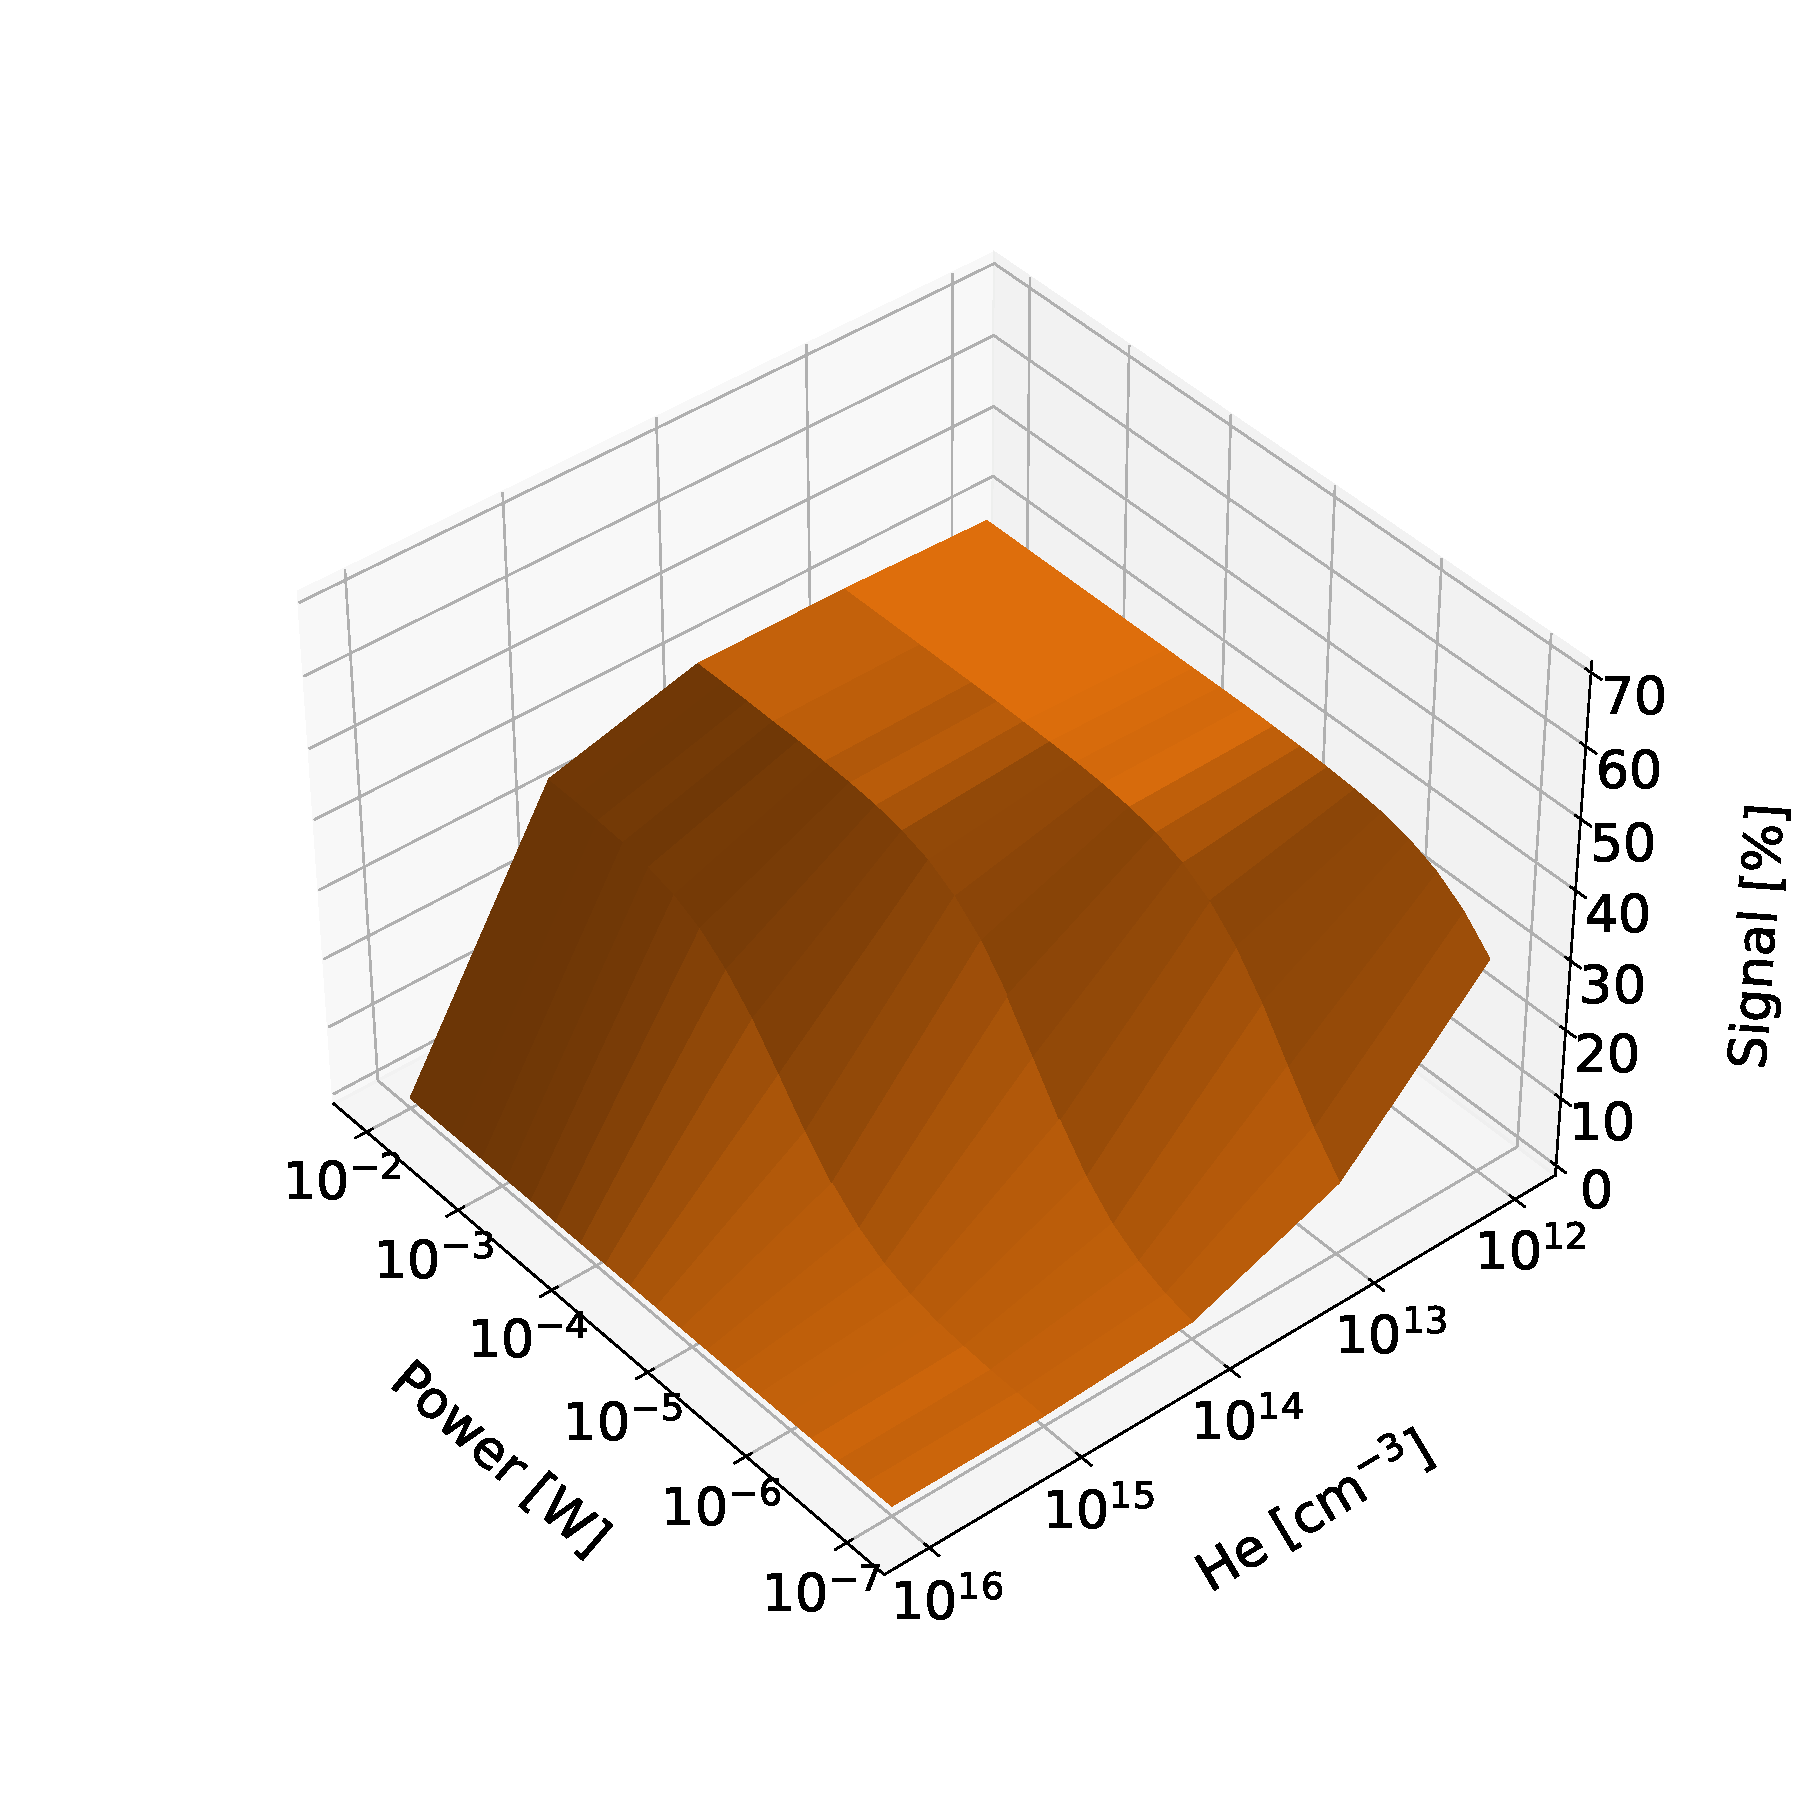
\includegraphics[width=1\textwidth]{figures/simulations/ROSAA/f-power_1e-7-1e-2/k3_branch_0.40.pdf}}{$k_{3_1}$ ratio $=0.4$}{}
    \hfill
    \Subfigure[0.3]{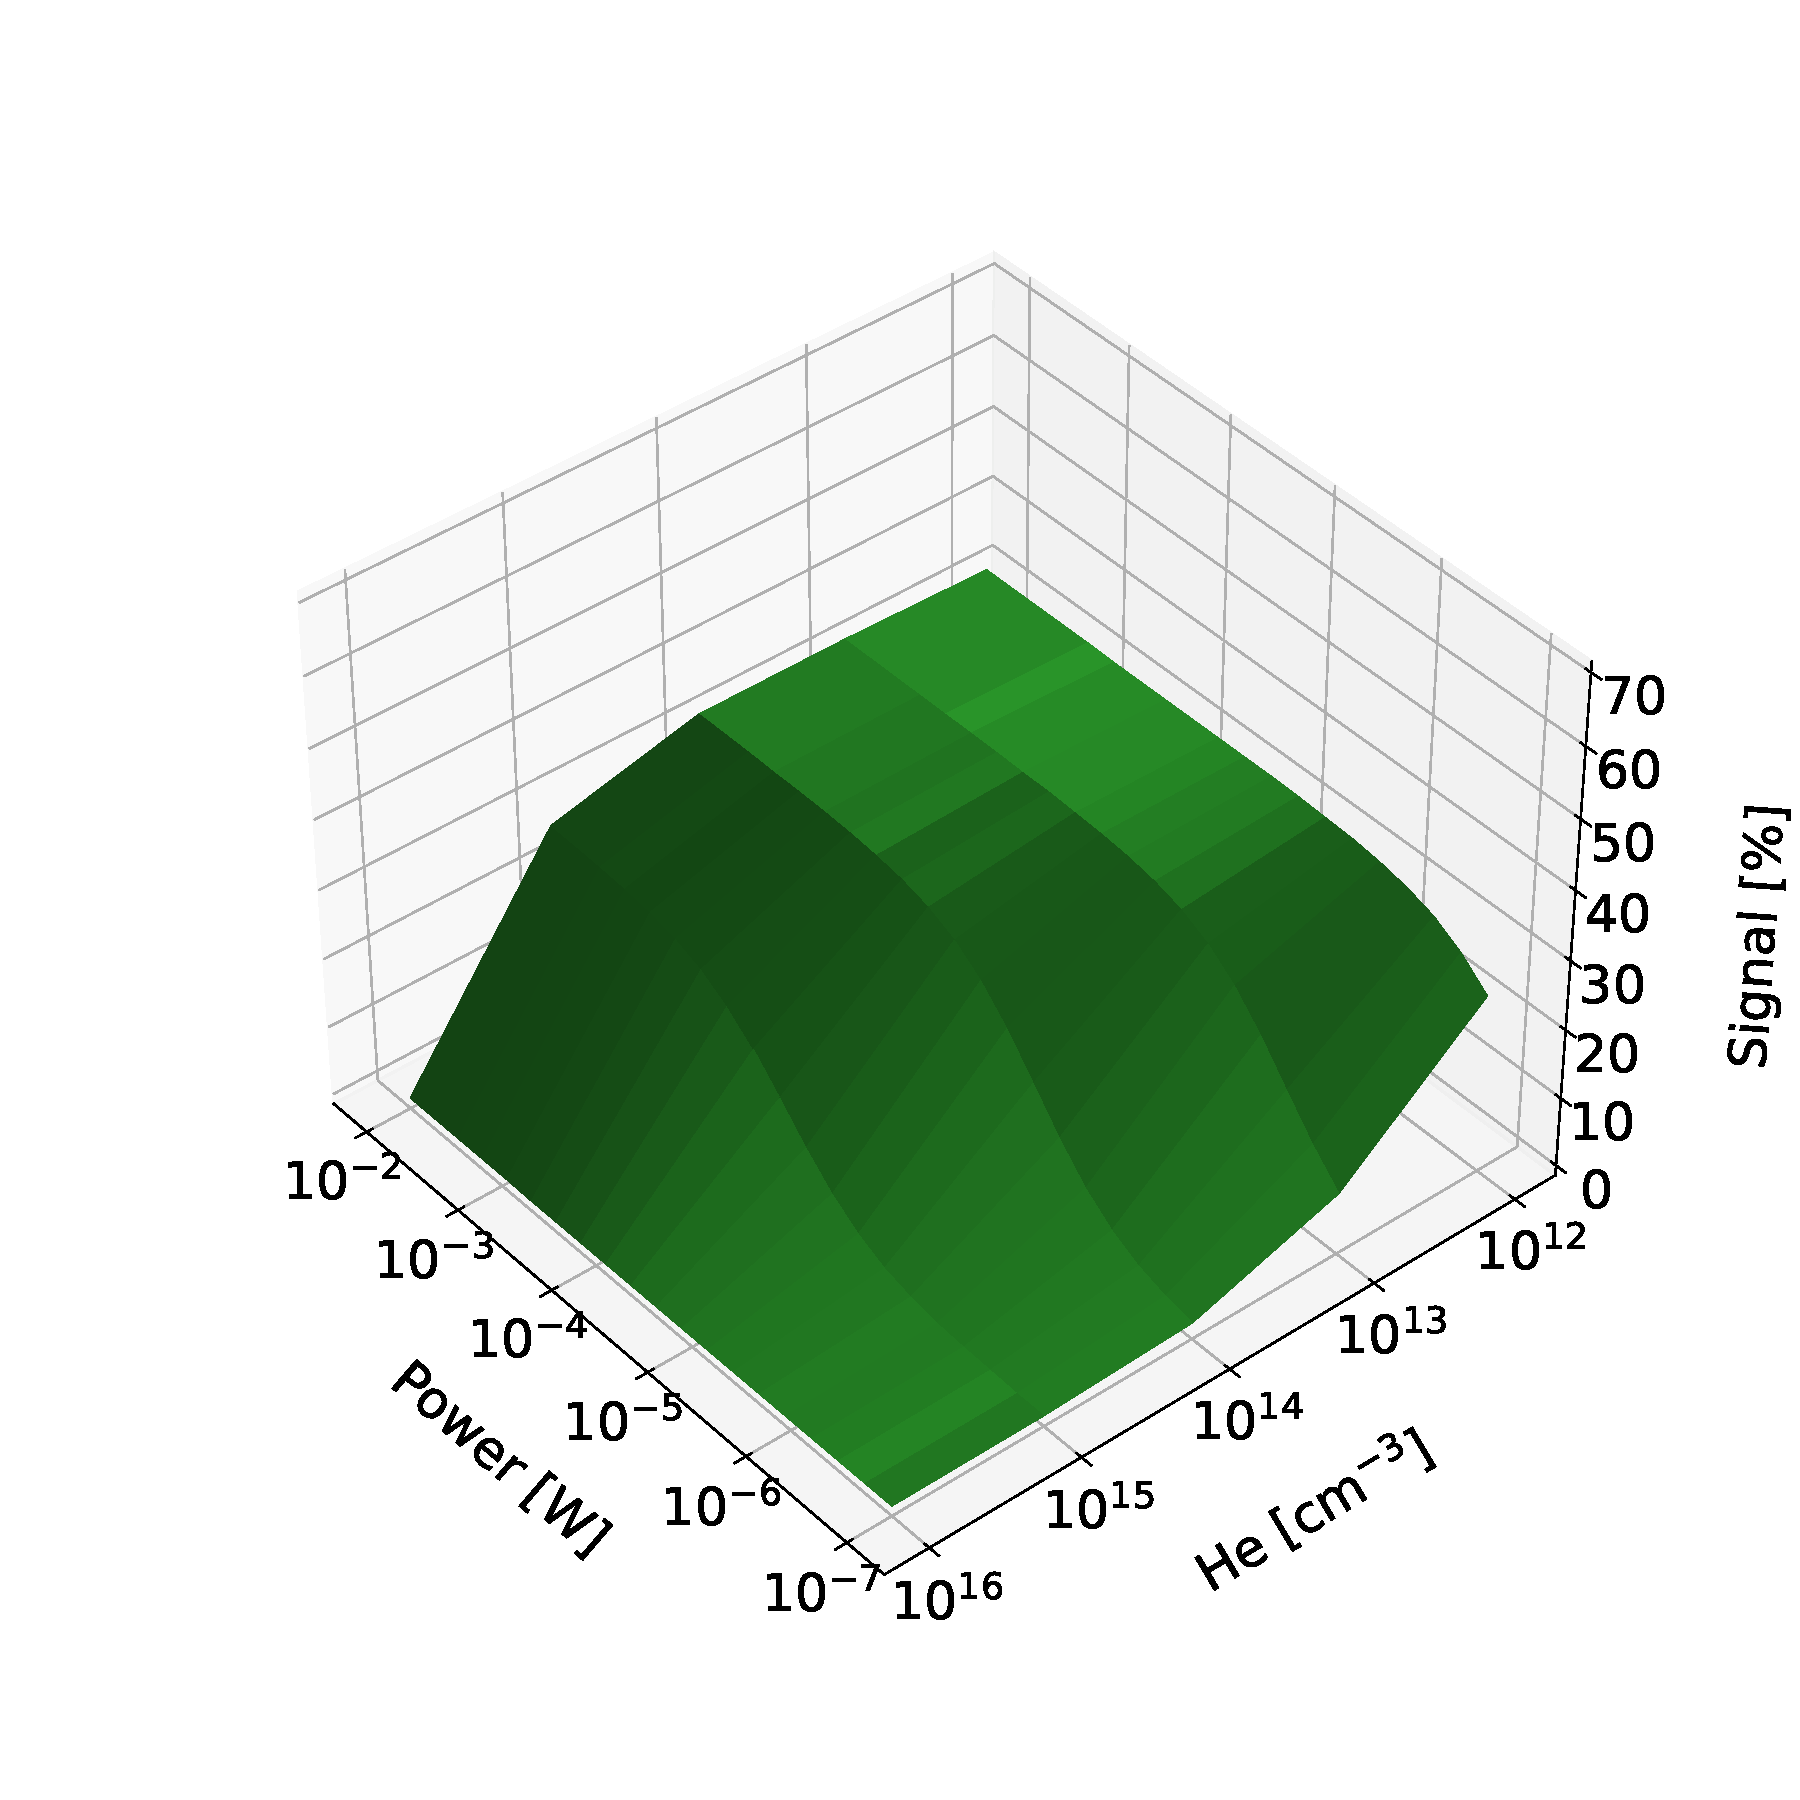
\includegraphics[width=1\textwidth]{figures/simulations/ROSAA/f-power_1e-7-1e-2/k3_branch_0.50.pdf}}{$k_{3_1}$ ratio $=0.5$}{\label{fig:thz:all-simulation:0.5a}}
    \hfill
    \Subfigure[0.3]{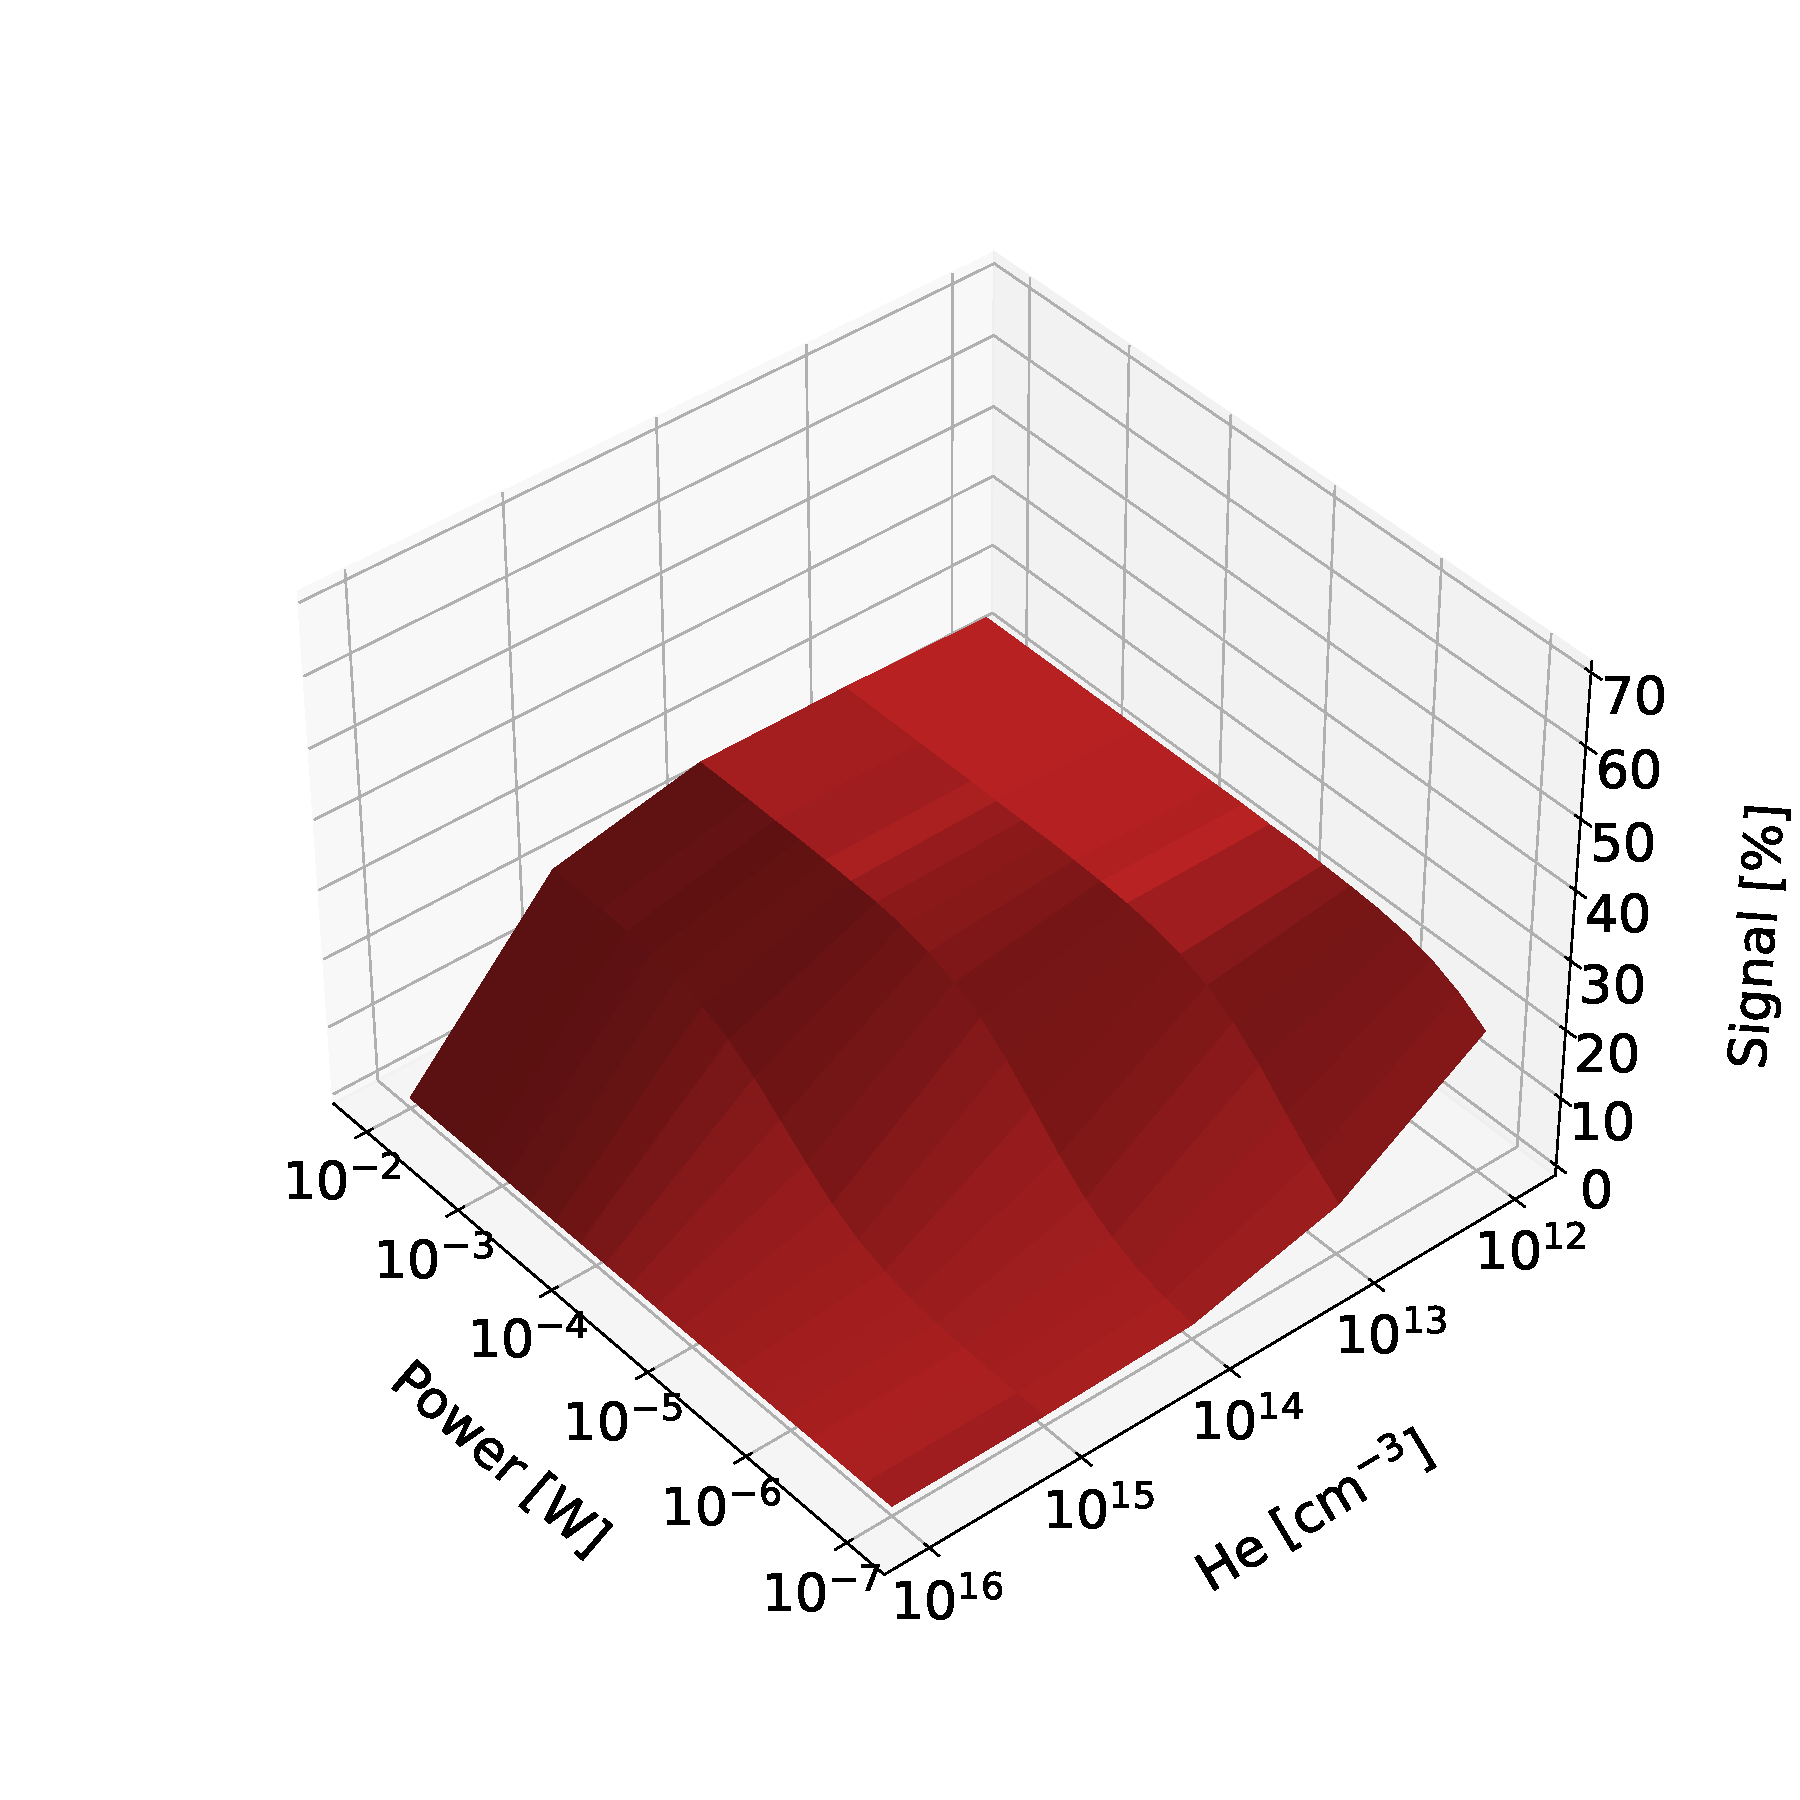
\includegraphics[width=1\textwidth]{figures/simulations/ROSAA/f-power_1e-7-1e-2/k3_branch_0.60.pdf}}{$k_{3_1}$ ratio $=0.6$}{}
    \hfill
    \Subfigure[0.3]{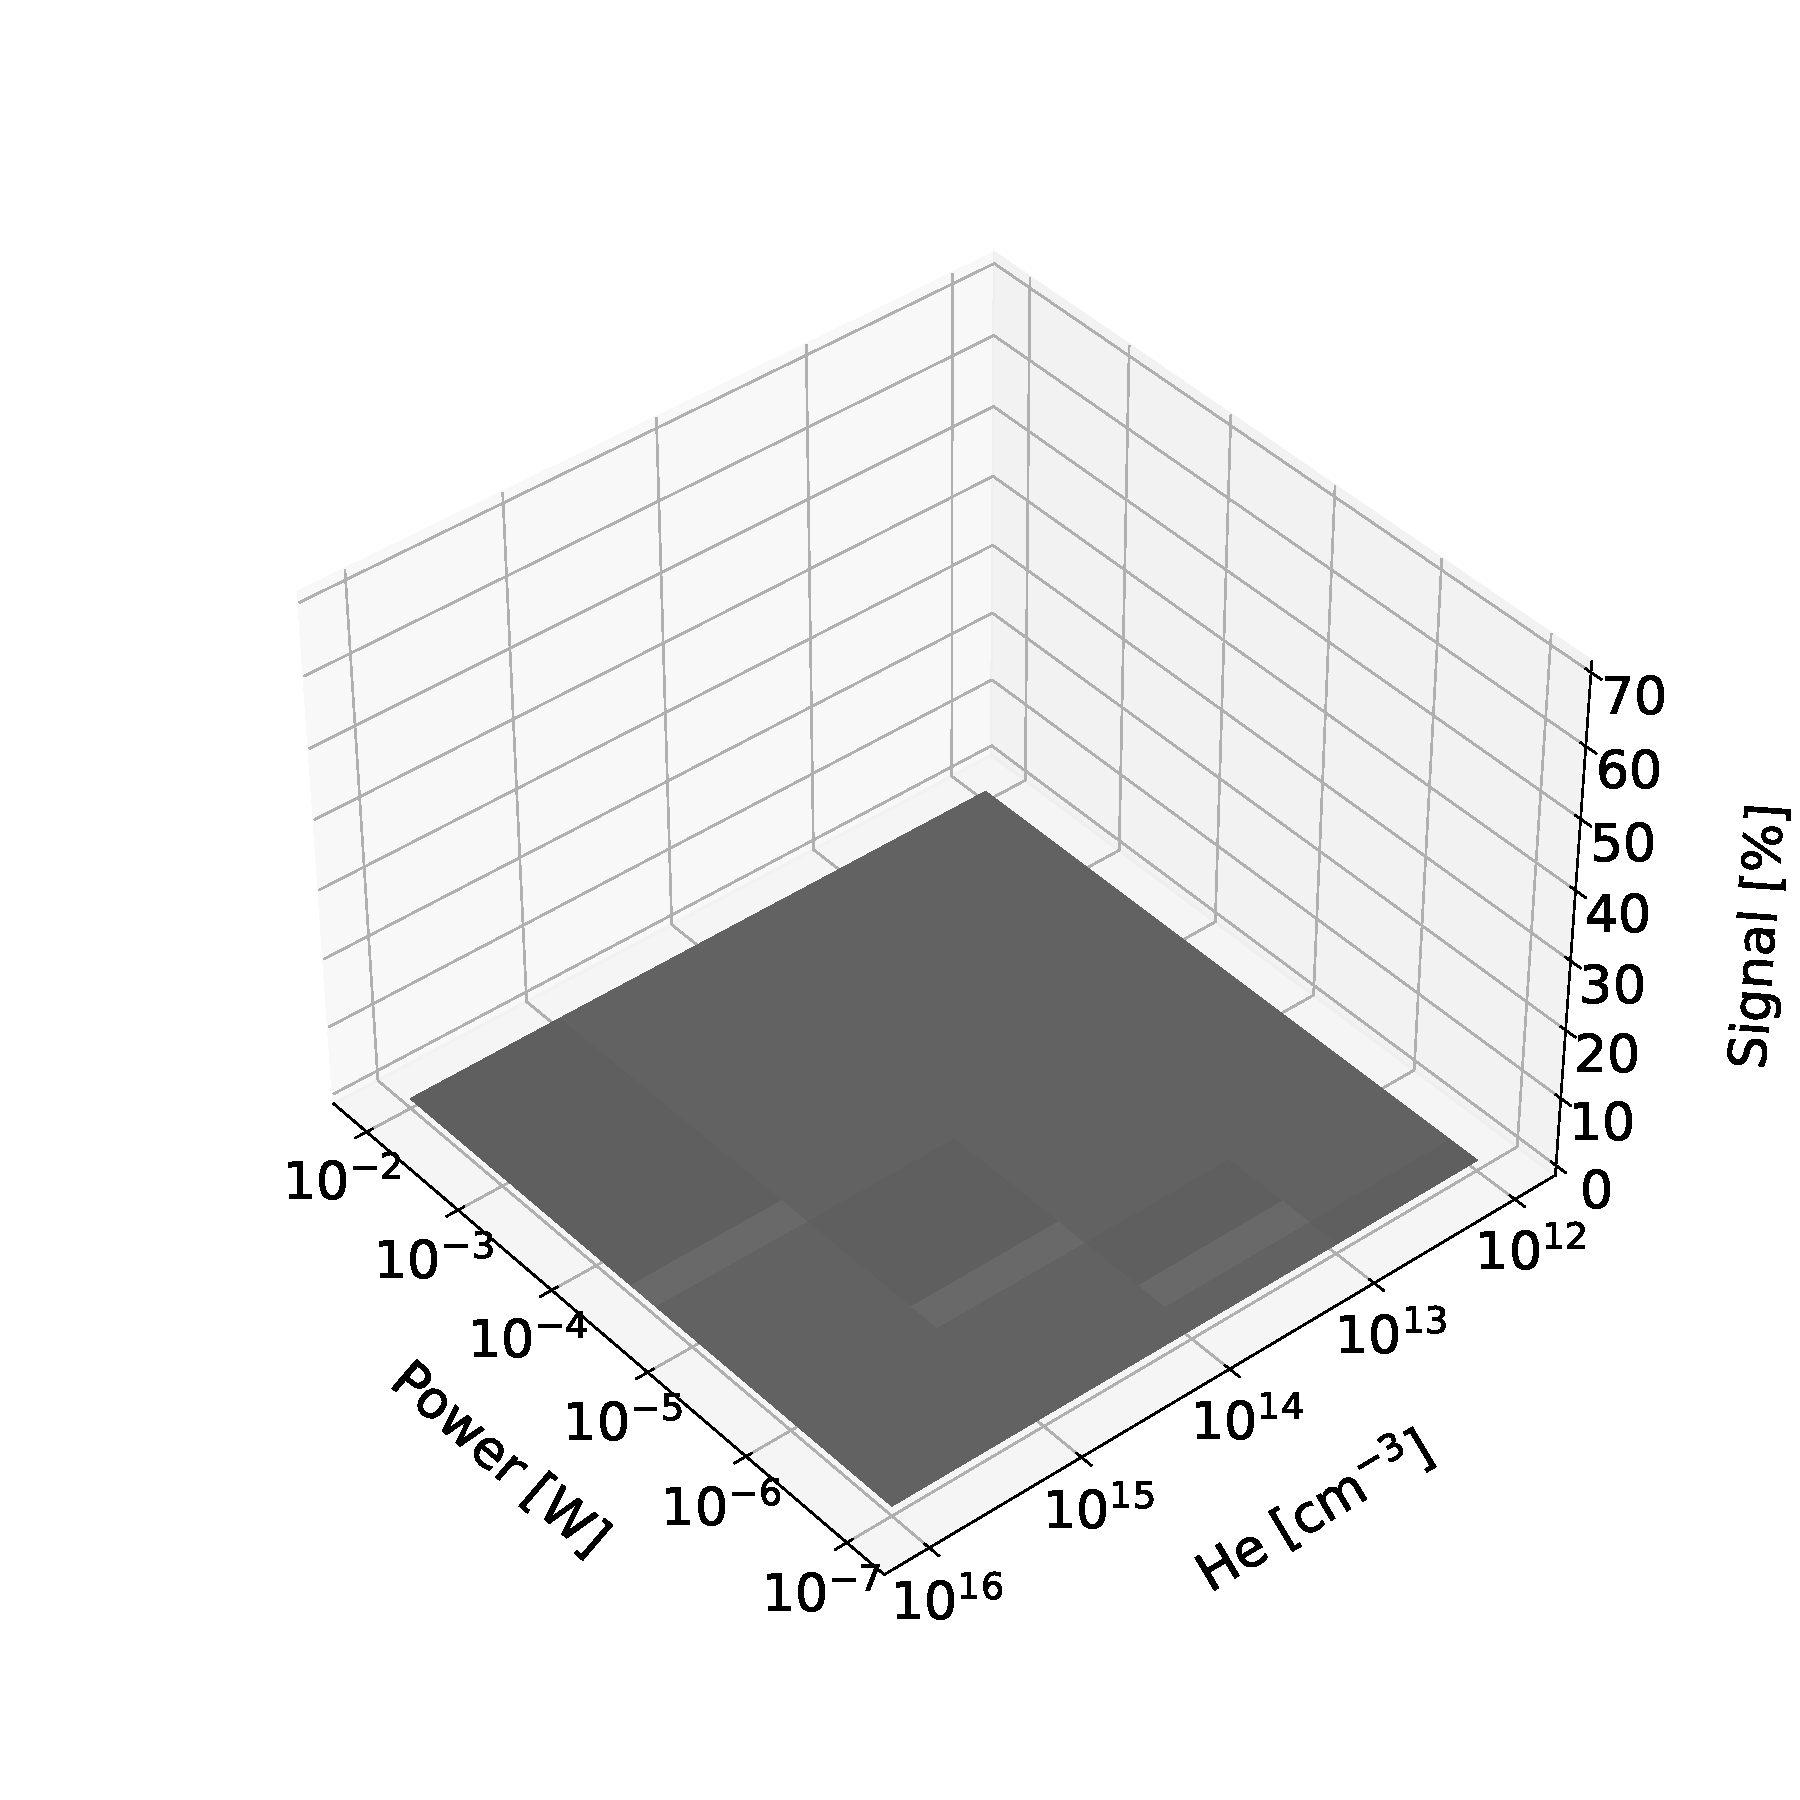
\includegraphics[width=1\textwidth]{figures/simulations/ROSAA/f-power_1e-7-1e-2/k3_branch_1.00.pdf}}{$k_{3_1}$ ratio $=1$}{\label{fig:thz:all-simulation:0.1a}}
    \hfill
    \Subfigure[0.3]{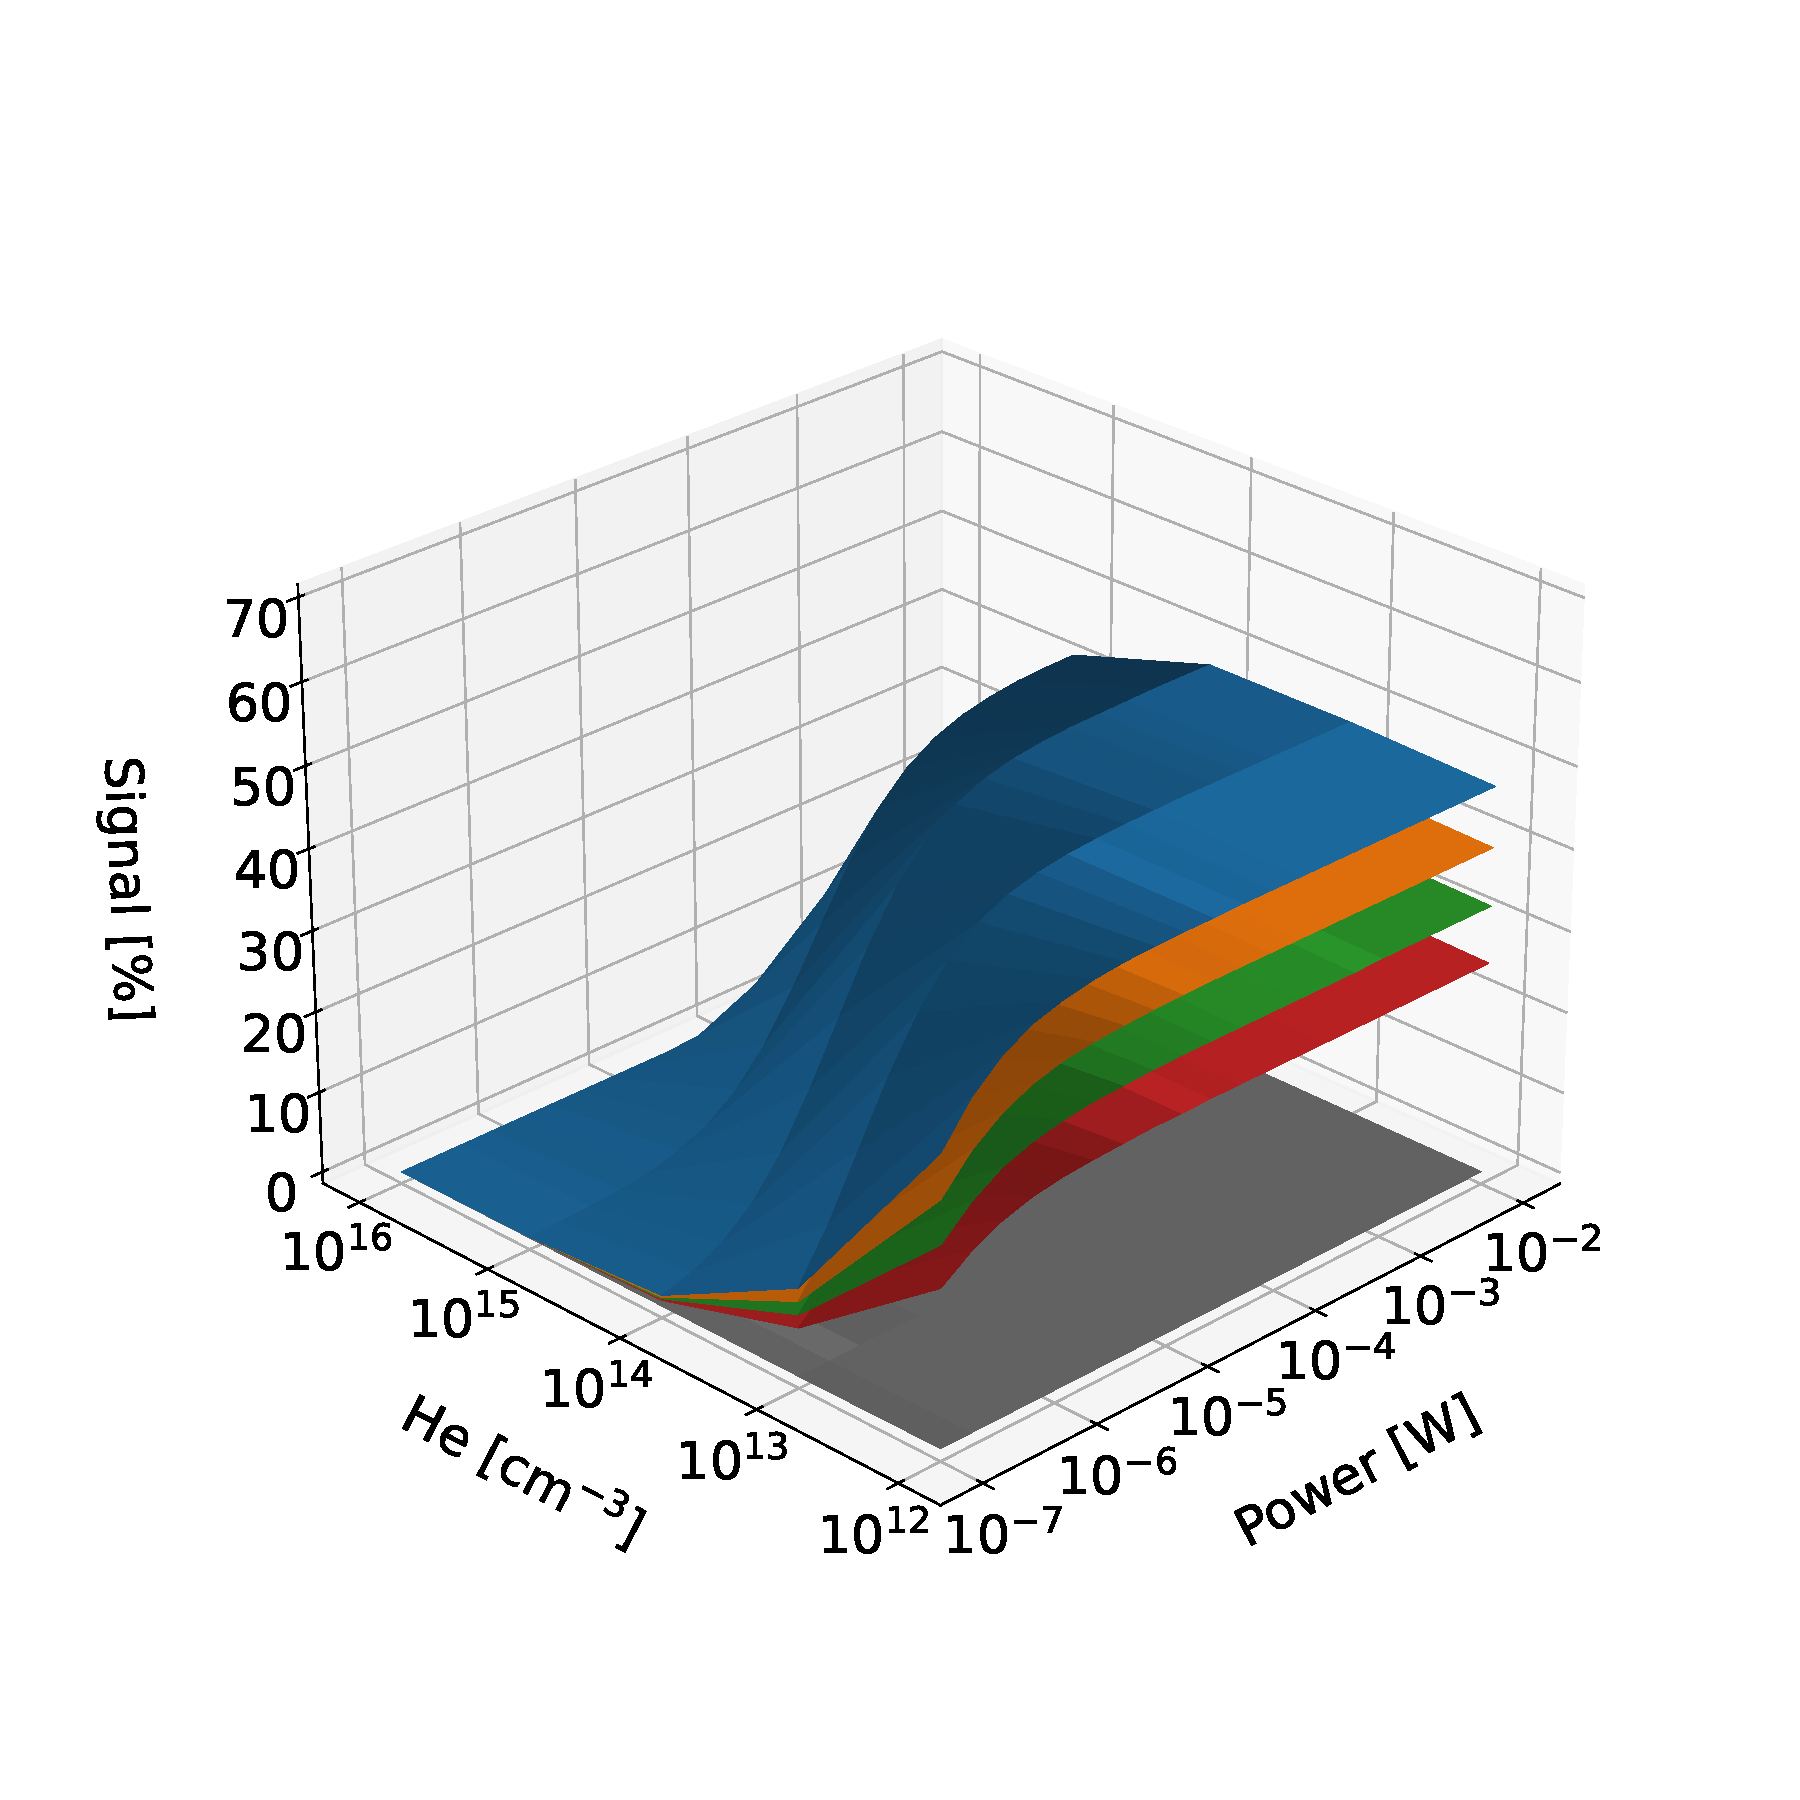
\includegraphics[width=1\textwidth]{figures/simulations/ROSAA/f-power_1e-7-1e-2/combined.pdf}}{combined}{}
    
    \caption{Numerical simulation of ROSAA process with computed signal intensities as a function of radiation power, $10^{-7} - 10^{-2}$ W, He number density, $10^{12} - 10^{16}$ \percc, and $k_{3_1}$ ratio, $0.3-1$, at 600 ms trap duration and T$_{coll}=7(1)$ K temperature. The captions of subplots (a)-(e) indicate the respective $k_{3_1}$ ratio value. (f) as captioned, shows the combined plots of (a)-(e).}
    \label{fig:thz:all-simulation}
\end{figure}
